\chapter{Scheduling Algorithm}
This section describes how the central server distributes jobs to work machines: the \textit{scheduling algorithm}.
Put briefly, the scheduling algorithm takes a list of jobs and decides which ones to run on the available work machines.
The scheduling algorithm has the following goals:
\begin{itemize}
  \item Keep work machines busy: there should be no idle work machines if there are pending jobs that could be run on them.
  \item Consider user-set job priorities: jobs with high user-set priorities should be worked on first.
  \item Prefer older jobs: older jobs should be worked on before newer jobs (assuming equal user-set priorities).
  \item Jobs should not be starved: even jobs with a low user-set priority should get to run eventually.
\end{itemize}
The scheduling algorithm operates under the following conditions:
\begin{itemize}
  \item Jobs arrive at unforeseen times.
  \item Time required to complete jobs is unknown.
  \item Jobs cannot be transferred from one work machine to another.
  \item Jobs cannot be restarted once they have been canceled.
  \item Job preemption is limited: if a job is paused it has to be kept either in physical memory or virtual memory (swap file).
  \item Some jobs cannot be paused due to software licensing restrictions.
\end{itemize}
The scheduling algorithm takes the following parameters as input:
\begin{itemize}
  \item List of pending jobs.
  \item List of running/paused jobs per work machine.
  \item Amount of work machine specific resources: CPU threads, memory, etc.
  These resources can typically be freed by pausing jobs.
  \item Amount of work machine unspecific resources: software licenses.
  Whether these resources can be freed by pausing jobs depends on the software.
  \item Size of work machine swap files.
  This resource is used exclusively for holding paused jobs.
  It has no influence on running jobs.
\end{itemize}
The scheduling algorithm reevaluates which jobs to run when
\begin{itemize}
  \item a new job arrives or
  \item a job finishes running or
  \item at a periodic time interval.
\end{itemize}
When the scheduling algorithm reevaluates which jobs to run it calculates an \textit{effective priority} $p$ for each job.
This effective priority $p$ depends on the following parameters:
\begin{itemize}
  \item the user-set job priority $p_0$.
  \item the current wall time $t$.
  \item the wall time at which the job was scheduled $t_0$.
  \item some positive constant $C$.
\end{itemize}
The effective priority $p_0$ can then be calculated as follows:
\begin{equation}
p = p_0 + C \cdot (t - t_0).
\end{equation}
Given the effective priorities for each job the scheduling algorithm then performs the following steps:
\begin{enumerate}
  \item If there are pending urgent jobs:
  Assign urgent jobs to work machines until urgent jobs or resources run out.
  Jobs are added in the order of their effective priority $p$ (oldest to newest).
  Non-urgent running jobs will be paused if possible and necessary to run more urgent jobs.
  \item If there are paused non-urgent jobs:
  Resume non-urgent jobs until paused non-urgent jobs or resources run out.
  Jobs are resumed in the order of their effective priority $p$.
  Running jobs with equal or lower effective priority $p$ will be paused if possible and necessary to run jobs with higher effective priority $p$.
  \item If there are pending non-urgent jobs:
  Assign pending non-urgent jobs to work machines until pending non-urgent jobs or resources run out.
  Jobs are assigned to work machines in the order of their effective priority $p$.
  By default, the scheduling algorithm will \textbf{not} pause running jobs to free up resources to run non-urgent jobs.
  However, this behavior changes once the effective priority $p$ of a non-urgent job reaches a certain threshold:
  once the threshold is reached the scheduling algorithm will begin to pause non-urgent running jobs with lower effective priority $p$ if possible and necessary to run the job with an effective priority $p$ above the threshold.
\end{enumerate}

\begin{figure}
  \centering
  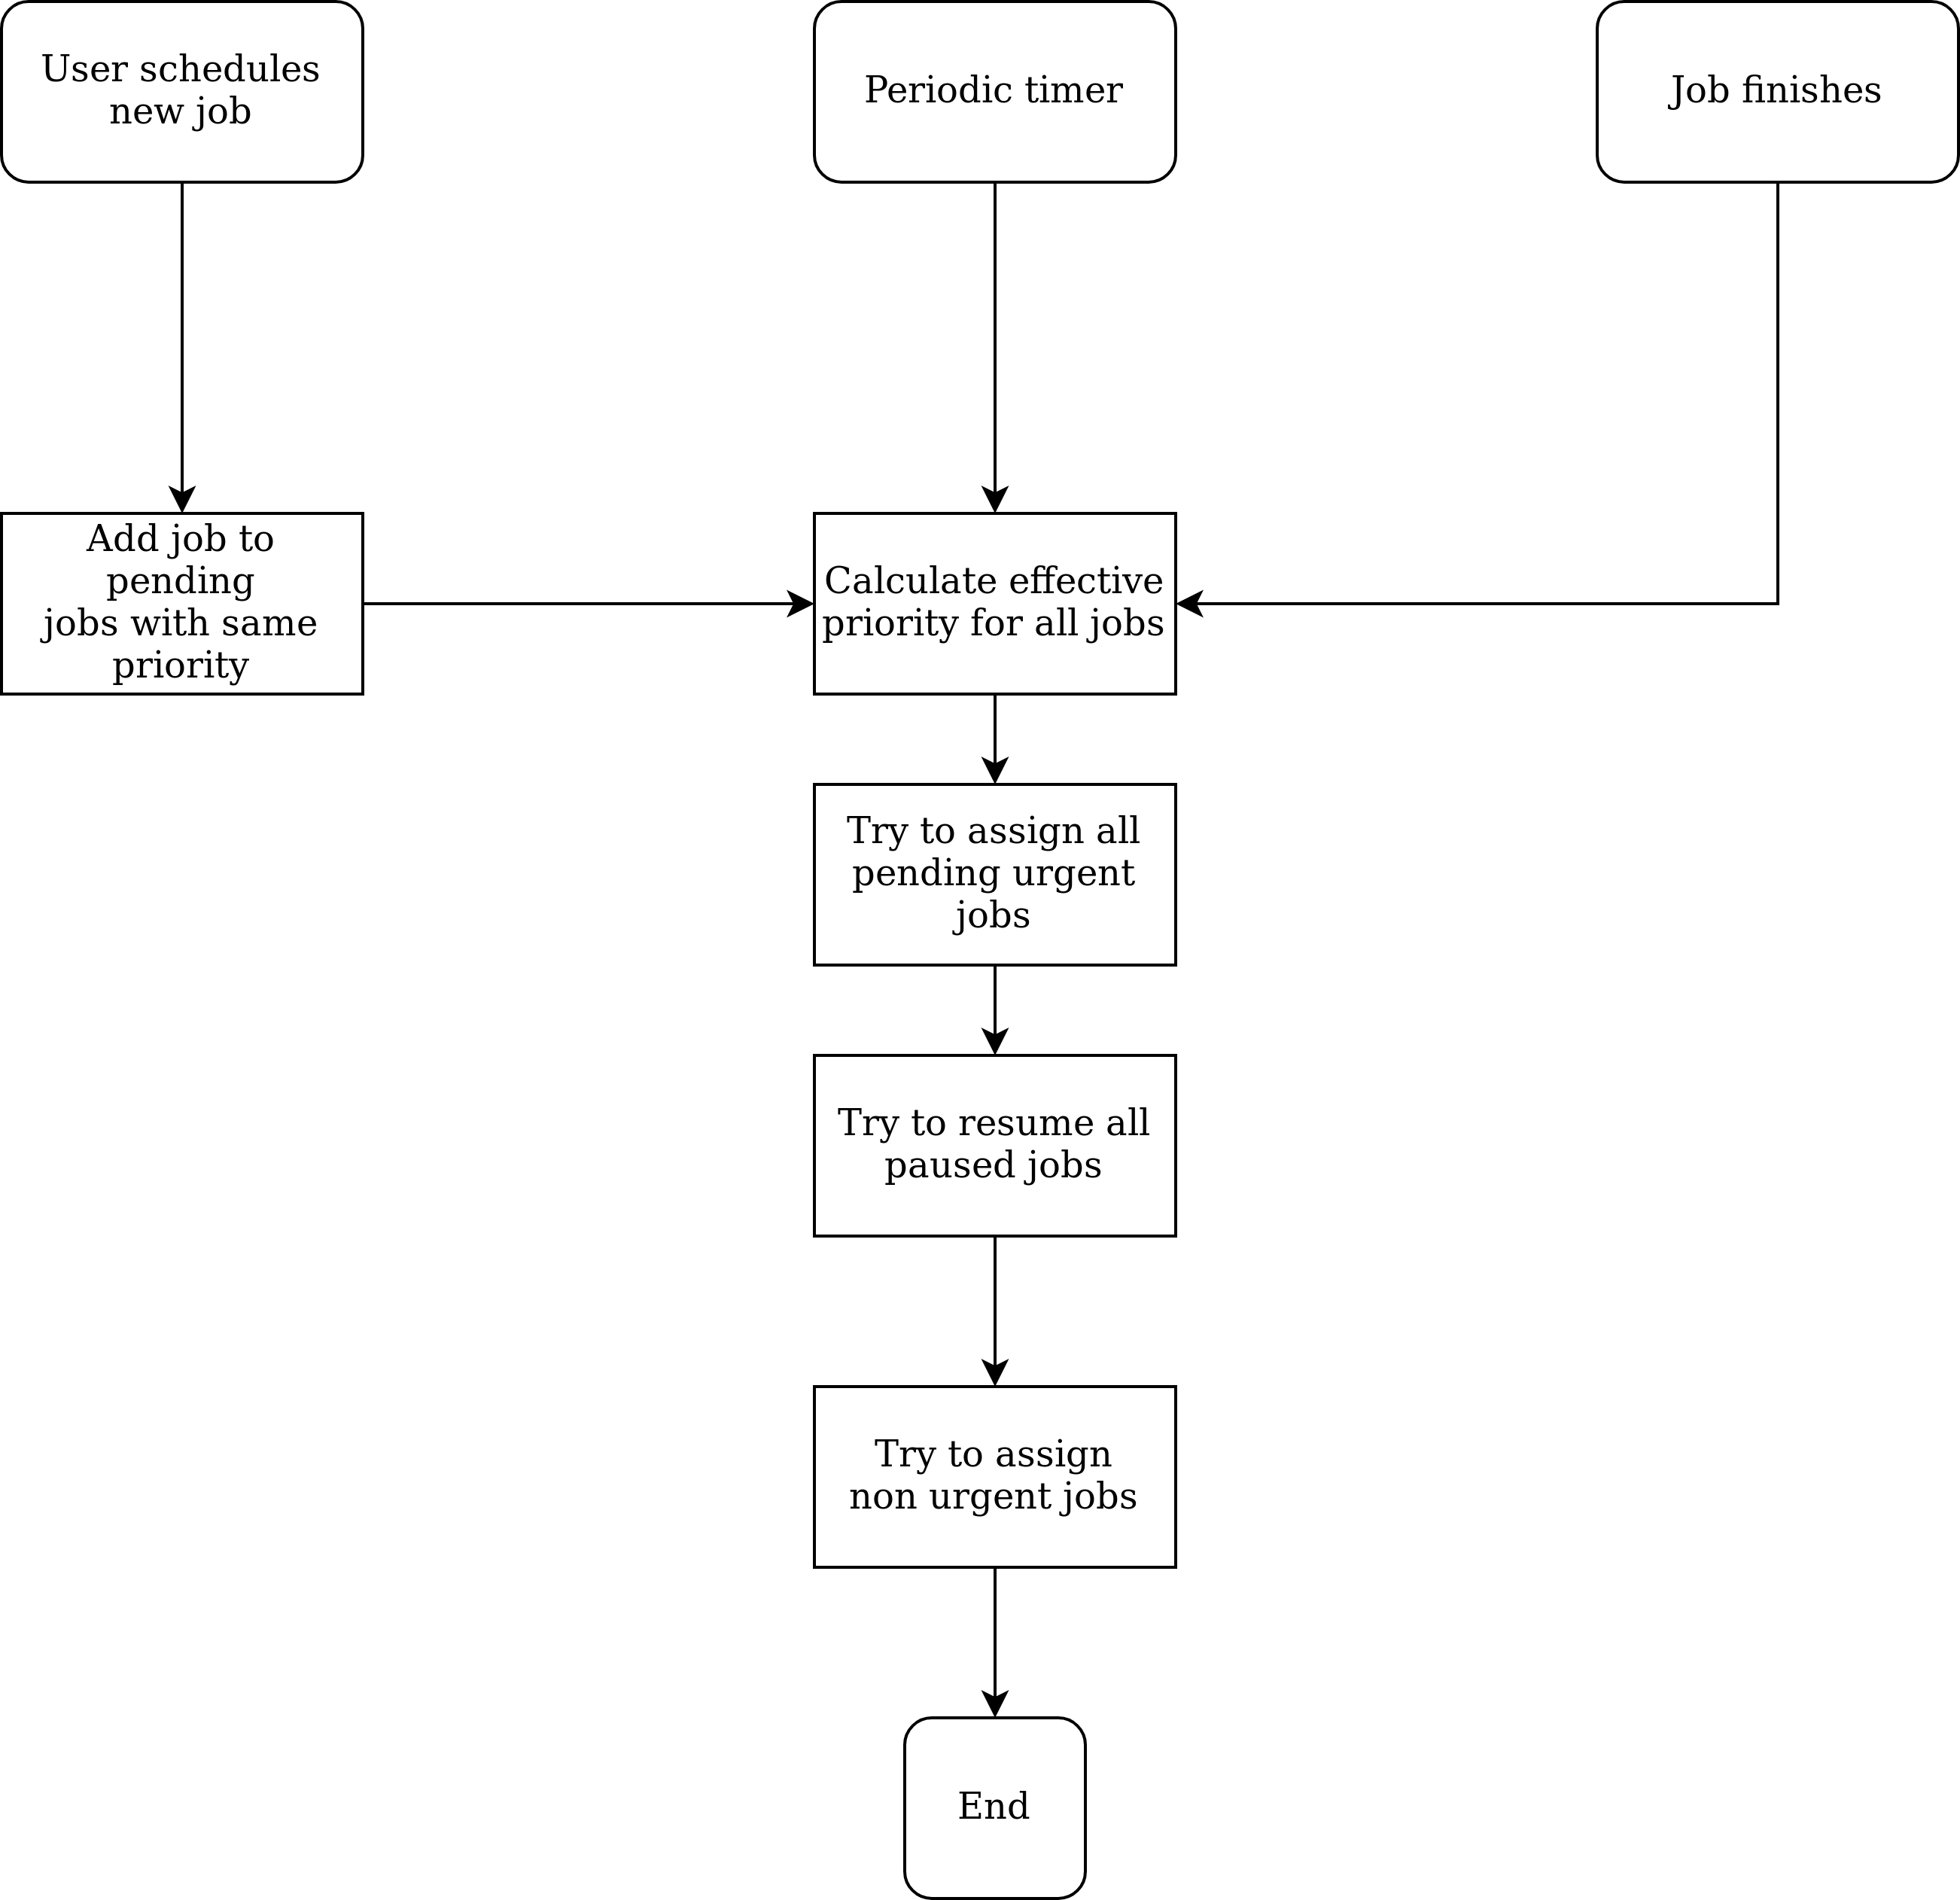
\includegraphics[width=0.9\textwidth]{./customer/diagrams/png/main-idea.png}
  \caption{This diagram depicts one iteration of the scheduling algorithm.
    The effective priorities of jobs are reevaluated when the set of runnable jobs changes or after a periodic time interval.
    The scheduling algorithm then attempts to assign jobs to work machines.
    First it tries to assign all pending urgent jobs, followed by all paused non-urgent jobs, and lastly all pending non-urgent jobs.
    Inside the aforementioned three steps the scheduling algorithm processes jobs in descending order of their effective priority (high priority first).
    Diagrams for how the scheduling algorithm decides if a single job can be assigned/resumed are shown in graphics: \hyperref[urgent]{Figure 2} \hyperref[paused]{Figure 3} \hyperref[non-urgent]{Figure 4}}
\end{figure}
\begin{figure}
  \centering
  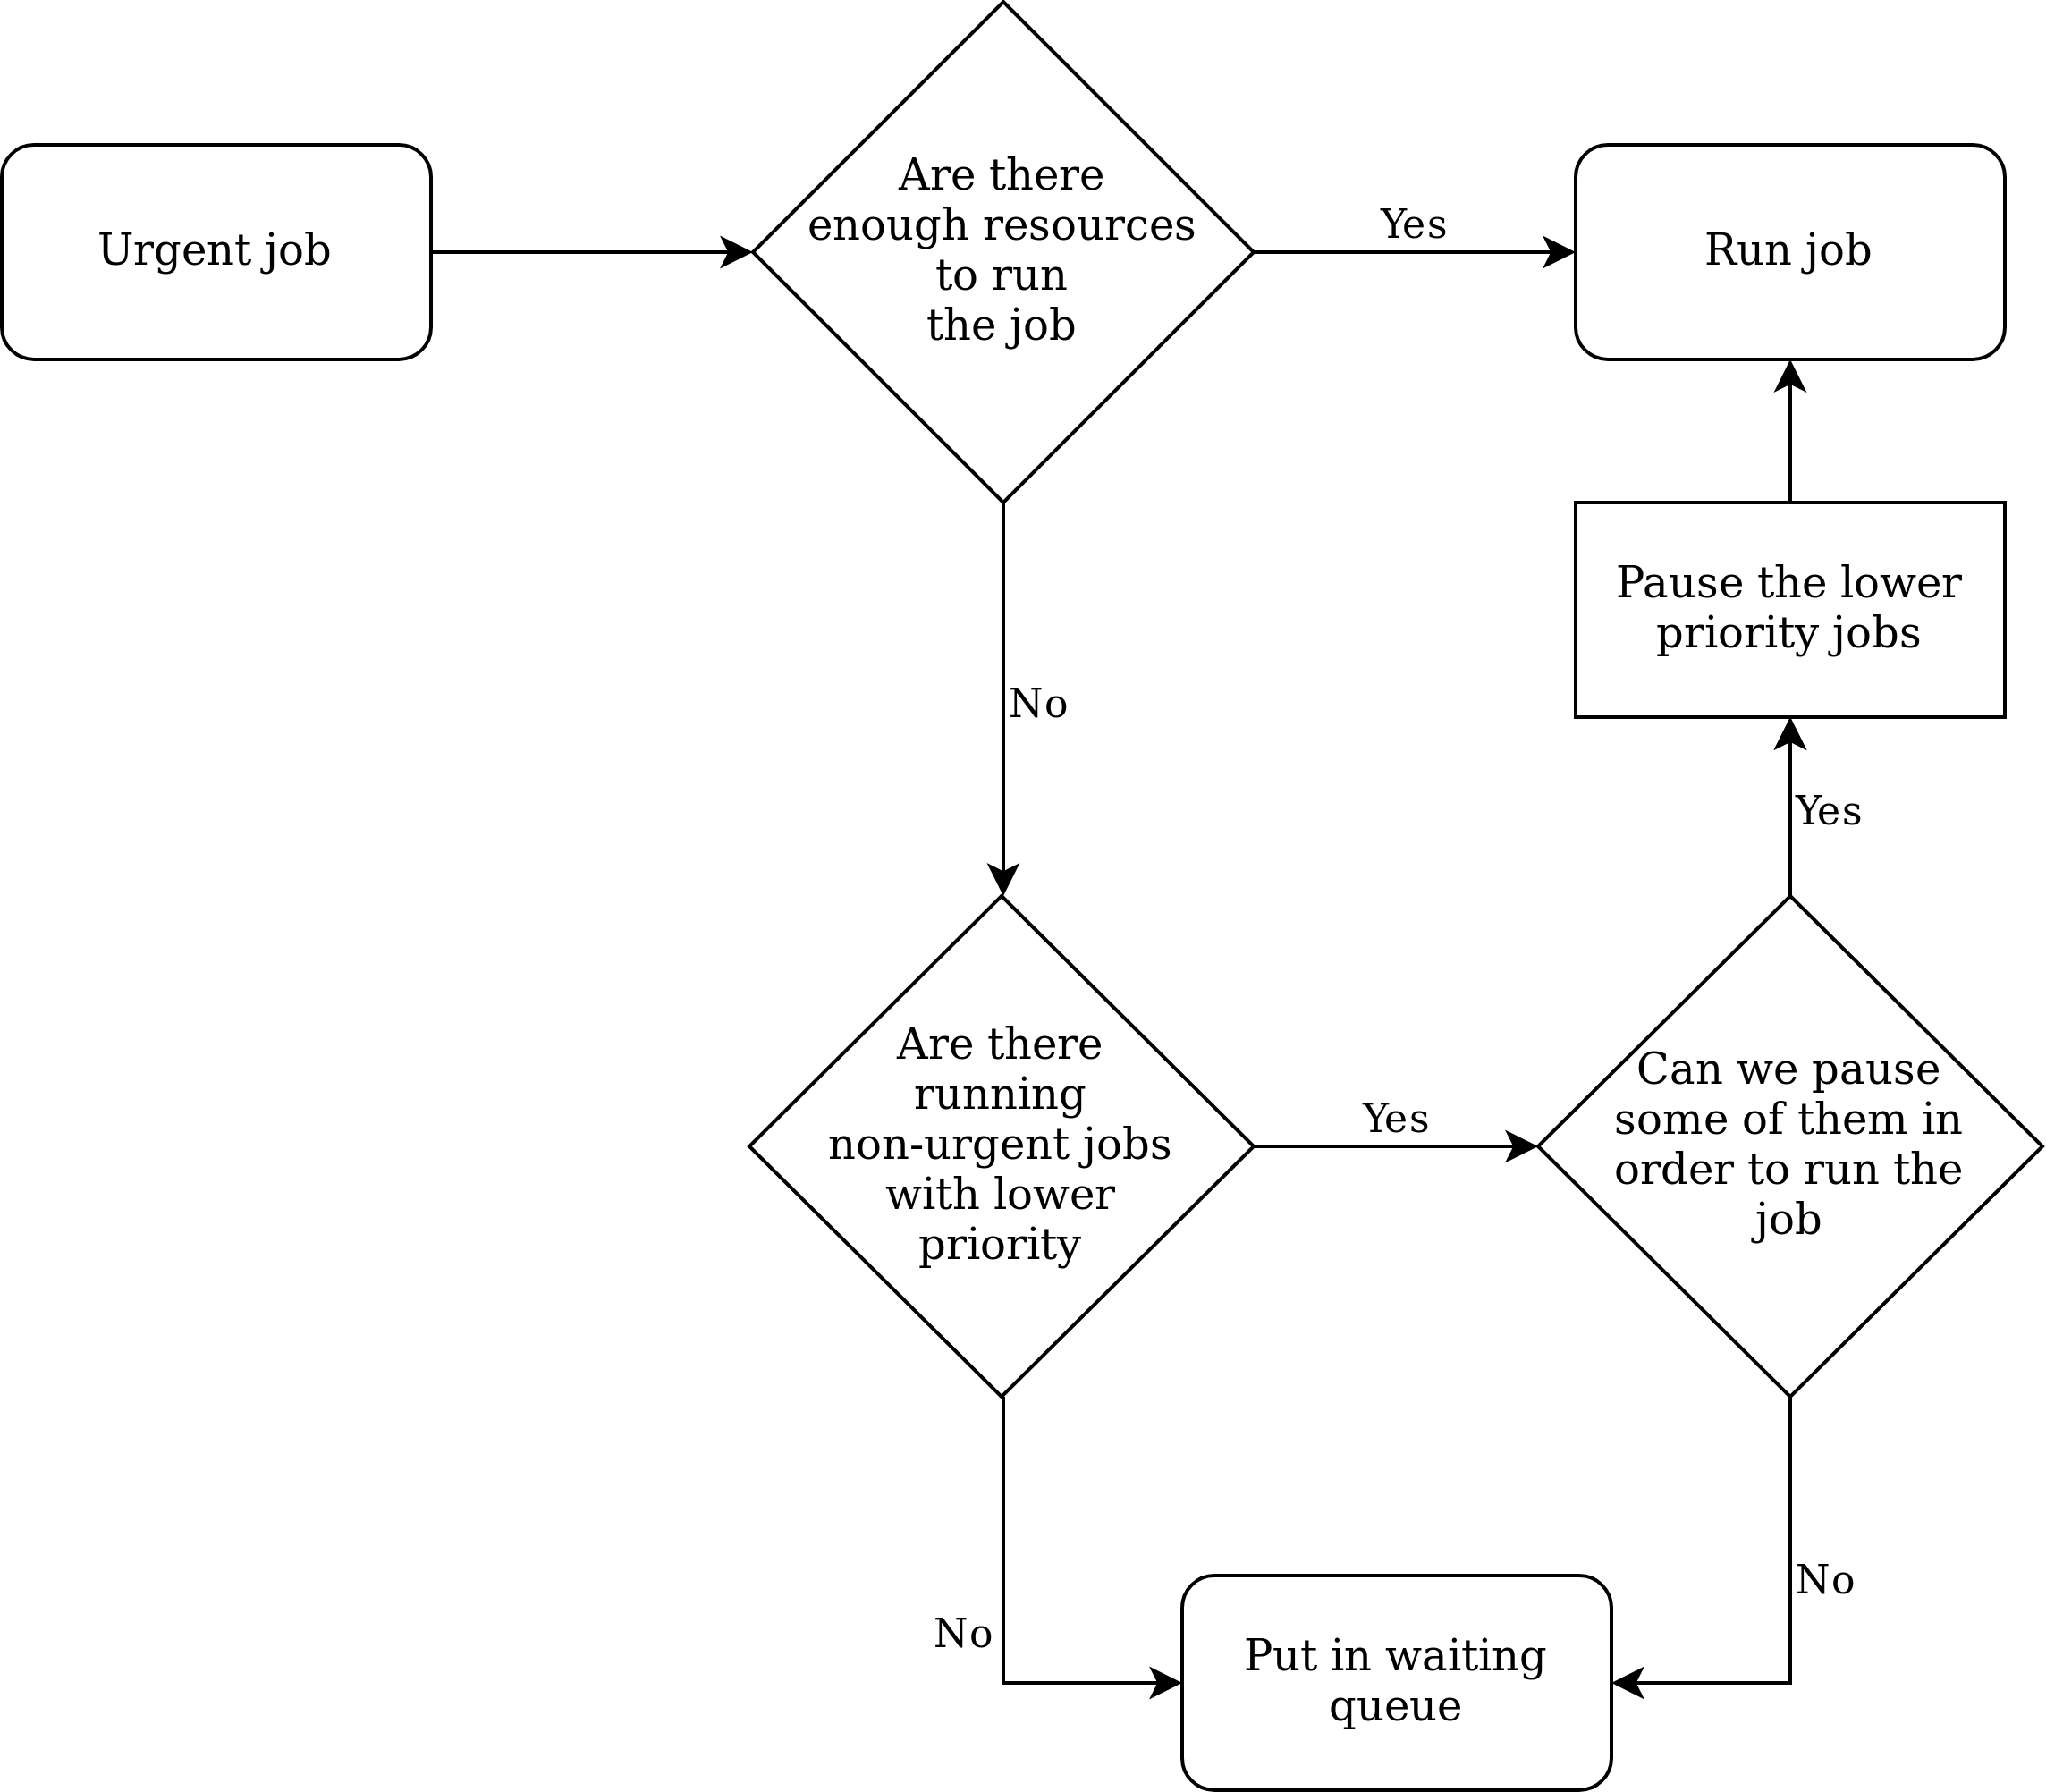
\includegraphics[width=\textwidth]{./customer/diagrams/png/urgent-job.png}
  \caption{This diagram depicts how the algorithm processes an urgent job.
  Non-urgent jobs will be paused to free up resources for the urgent job (if possible).}
  \label{urgent}
\end{figure}
\begin{figure}
  \centering
  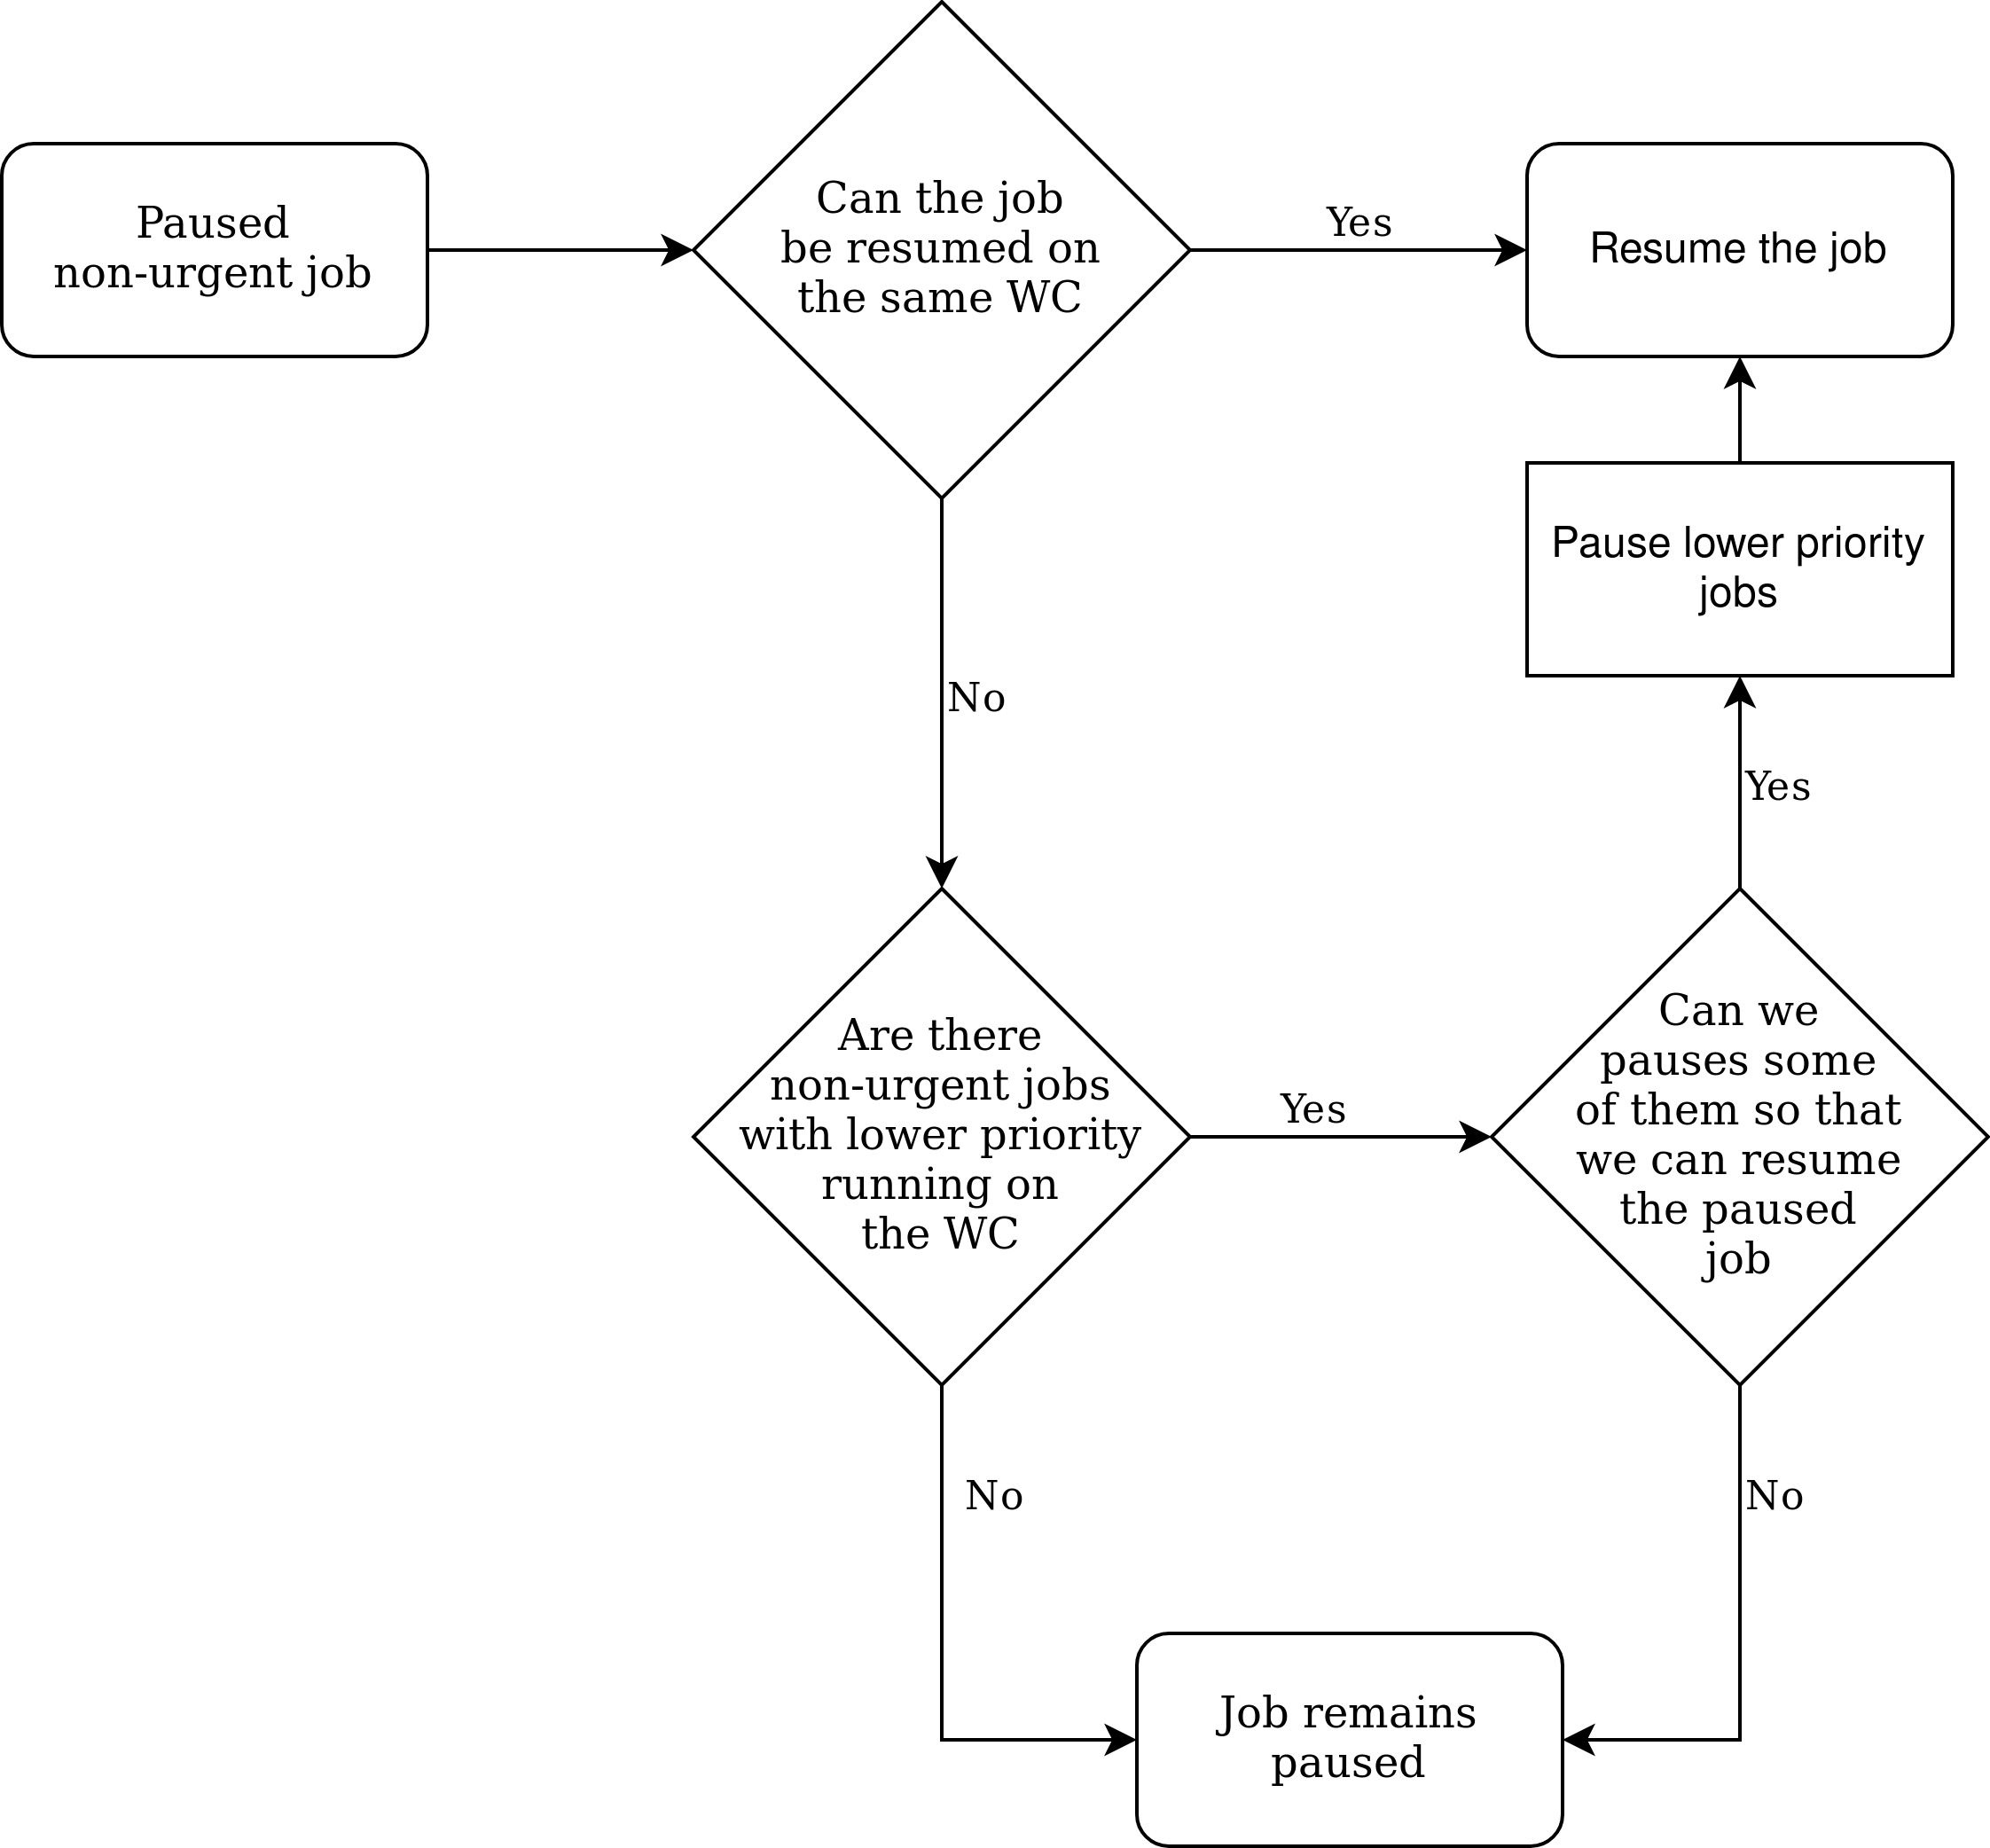
\includegraphics[width=\textwidth]{./customer/diagrams/png/paused-job.png}
  \caption{This diagram depicts how the algorithm processes a paused non-urgent job.
  Non-urgent jobs will be paused to free up resources for the paused job (if possible).}
  \label{paused}
\end{figure}
\begin{figure}
  \centering
  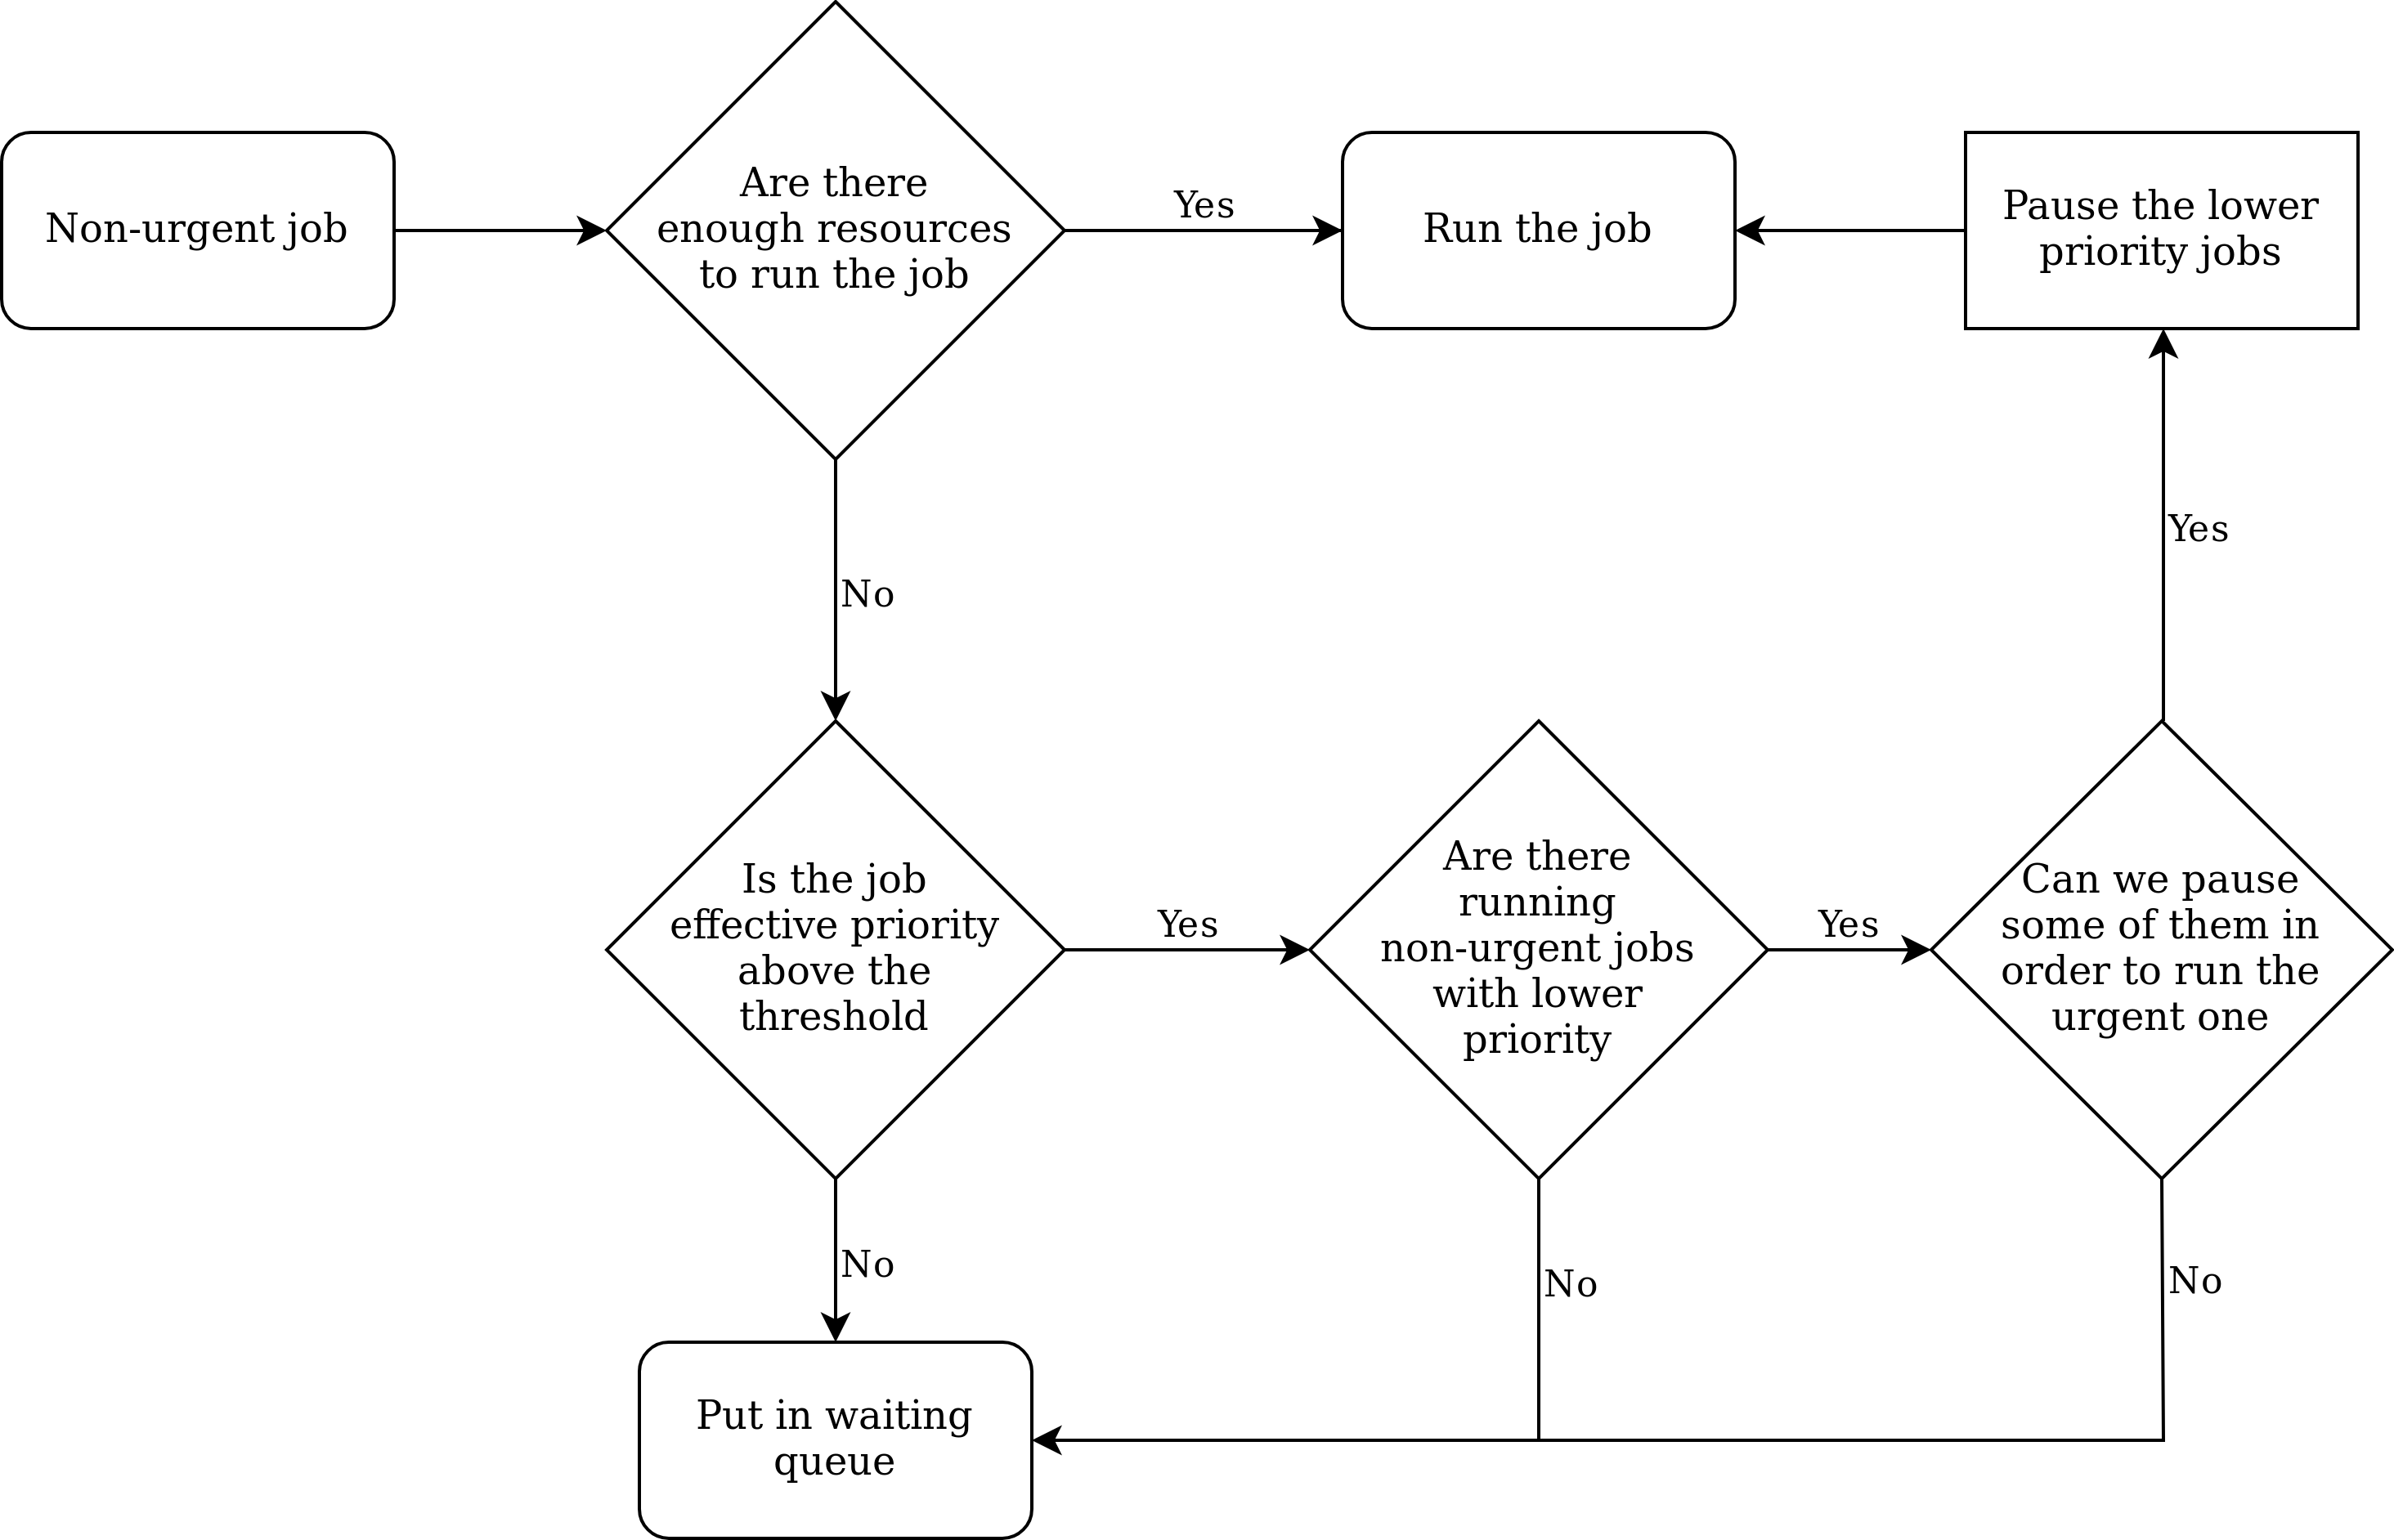
\includegraphics[width=\textwidth]{./customer/diagrams/png/non-urgent-job.png}
  \caption{This diagram depicts how the algorithm processes a pending non-urgent job.
  By default the algorithm will not pause running jobs to free up resources to run non-urgent jobs.
  But if the effective priority of the job reaches a threshold, the non-urgent job will follow the same steps as a urgent job.}
  \label{non-urgent}
\end{figure}

